\documentclass[10pt, aspectratio=169]{beamer}
% Shared setup for every day of the course.
\usetheme[progressbar=frametitle, numbering=fraction, block=fill]{metropolis}
\usepackage[T1]{fontenc}
\usepackage[utf8]{inputenc}
\usepackage{lmodern}
\usepackage{amsmath, amssymb, bm, booktabs, graphicx, xcolor}
\usepackage{tikz}
\usetikzlibrary{arrows.meta, positioning, calc, shapes.geometric}

\graphicspath{{figures/}}

% --- colours -------------------------------------------------------------------------------------
\definecolor{accent}{HTML}{C0392B}
\definecolor{cool}{HTML}{2E6DB4}
\definecolor{muted}{HTML}{7A7A7A}
\definecolor{good}{HTML}{2E8B57}
\setbeamercolor{alerted text}{fg=accent}
\setbeamercolor{example text}{fg=cool}

% --- notation (follows the thesis' notation chapter) ---------------------------------------------
\newcommand{\given}{\,|\,}
\newcommand{\E}{\mathbb{E}}
\newcommand{\KL}[2]{D_{\mathrm{KL}}\!\left[#1\,\middle\|\,#2\right]}
\newcommand{\N}{\mathcal{N}}
\newcommand{\Hess}{\mathcal{H}}
\newcommand{\nats}{\,\text{nats}}
\DeclareMathOperator*{\argmin}{arg\,min}

% --- course devices ------------------------------------------------------------------------------
% \src{...}: where a claim or number comes from (thesis file and line, or a post-thesis note).
\newcommand{\src}[1]{\par\vfill\hfill{\scriptsize\color{muted}source: #1}}
% \wip: marks a post-thesis result.
\newcommand{\wip}{{\scriptsize\color{white}\colorbox{accent}{\,work in progress\,}}}
% \lesson{...}: the one sentence a frame exists to say.
\newcommand{\lesson}[1]{\begin{alertblock}{}\centering #1\end{alertblock}}
% a measurement story
\newenvironment{measured}[1]{\begin{exampleblock}{Measured: #1}}{\end{exampleblock}}

\author{Course built on the doctoral thesis of No\'e Zapata}
\institute{Montevideo, 30 November -- 4 December 2026}

% \cyclemap{n}: the course's five-stage cycle, stage n highlighted (1 room ... 5 memory).
\newcommand{\cyclemap}[1]{%
  \begin{tikzpicture}[
      st/.style={draw=muted, thick, rounded corners=3pt, fill=white, align=center,
                 minimum width=2.5cm, minimum height=0.8cm, font=\scriptsize, text=muted},
      on/.style={draw=accent, very thick, fill=accent!10, text=black, font=\scriptsize\bfseries},
      arr/.style={-{Stealth[length=2mm]}, thick, color=muted},
      s1/.style={}, s2/.style={}, s3/.style={}, s4/.style={}, s5/.style={}, s#1/.style={on}]
    \node[st, s1] (c1) at (90:1.9)   {estimate the room};
    \node[st, s2] (c2) at (18:2.6)   {localise; learn\\the body};
    \node[st, s3] (c3) at (-54:2.2)  {concepts fill\\the room};
    \node[st, s4] (c4) at (-126:2.2) {cross the door};
    \node[st, s5] (c5) at (162:2.6)  {new room;\\memory};
    \draw[arr] (c1) to[bend left=15] (c2); \draw[arr] (c2) to[bend left=15] (c3);
    \draw[arr] (c3) to[bend left=15] (c4); \draw[arr] (c4) to[bend left=15] (c5);
    \draw[arr] (c5) to[bend left=15] (c1);
  \end{tikzpicture}}


\title{A robot that acts to know}
\subtitle{Day 3 --- Belief in time}
\date{Wednesday 2 December}

\tikzset{bx/.style={draw, rounded corners=3pt, thick, align=center, font=\footnotesize,
                    minimum height=0.8cm, inner sep=3pt},
         lab/.style={font=\scriptsize},
         arr/.style={-{Stealth}, thick},
         obj/.style={draw, circle, thick, inner sep=0pt, minimum size=0.55cm, font=\scriptsize}}

\begin{document}

\maketitle

\begin{frame}{Yesterday: who holds a belief. Today: how long it lasts}
  \begin{columns}[c]
    \begin{column}{0.48\textwidth}
      \centering
      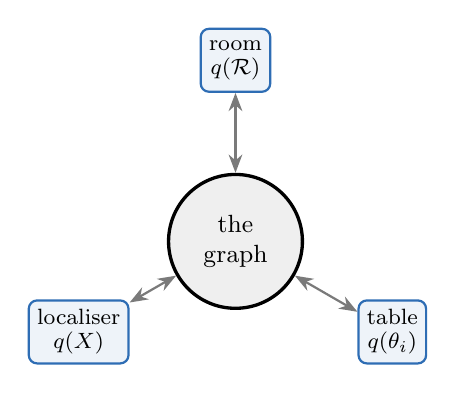
\begin{tikzpicture}
        \node[draw, circle, very thick, fill=muted!12, minimum size=1.7cm, align=center, font=\small] (g) at (0,0) {the\\graph};
        \foreach \a/\n/\s in {90/room/{$q(\mathcal R)$}, 330/table/{$q(\theta_i)$}, 210/localiser/{$q(X)$}} {
          \node[bx, draw=cool, fill=cool!8] (\n) at (\a:2.3) {\n\\[-0.1em]\s};
          \draw[{Stealth}-{Stealth}, thick, muted] (\n) -- (g);
        }
      \end{tikzpicture}\\[0.4em]
      \small one $F$, divided among owners; no thresholds
    \end{column}
    \begin{column}{0.48\textwidth}
      Every node on that graph is a belief with a life of its own. Today:
      \begin{itemize}
        \item how it \textbf{begins}: model comparison, not counting;
        \item how it \textbf{ends}: absence as evidence;
        \item how it \textbf{fades}: forgetting as inference;
        \item what it \textbf{stands on}: a room, a pose, and an assignment of evidence;
        \item and what happens when all of that shares \textbf{one error}.
      \end{itemize}
    \end{column}
  \end{columns}
\end{frame}

\begin{frame}{The life of an instance}
  \centering
  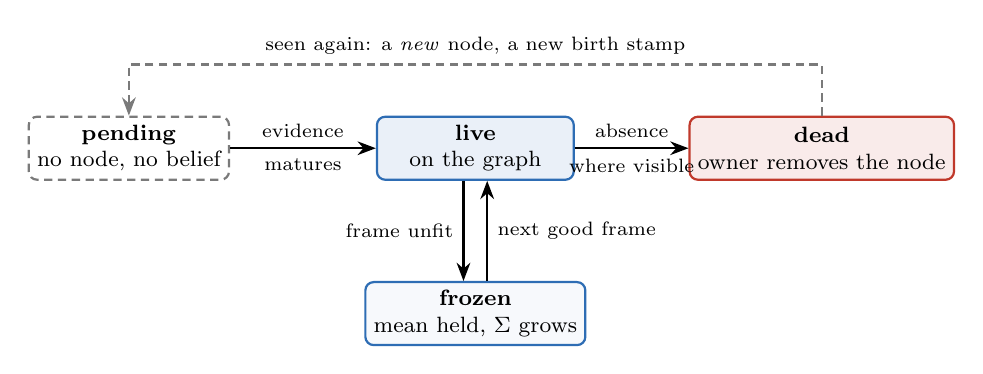
\begin{tikzpicture}
    \node[bx, draw=muted, densely dashed, minimum width=2.5cm] (p) at (0,0) {\textbf{pending}\\no node, no belief};
    \node[bx, draw=cool, fill=cool!10, minimum width=2.5cm] (l) at (4.4,0) {\textbf{live}\\on the graph};
    \node[bx, draw=cool, fill=cool!4, minimum width=2.5cm] (f) at (4.4,-2.1) {\textbf{frozen}\\mean held, $\Sigma$ grows};
    \node[bx, draw=accent, fill=accent!10, minimum width=2.5cm] (d) at (8.8,0) {\textbf{dead}\\owner removes the node};
    \draw[arr] (p) -- node[above, lab] {evidence} node[below, lab] {matures} (l);
    \draw[arr] (l) -- node[above, lab] {absence} node[below, lab] {where visible} (d);
    \draw[arr] (l.-110) -- node[left, lab] {frame unfit} (f.110);
    \draw[arr] (f.70) -- node[right, lab] {next good frame} (l.-70);
    \draw[arr, muted, densely dashed] (d.north) -- ++(0,0.65) -| node[above, lab, pos=0.25, text=black] {seen again: a \emph{new} node, a new birth stamp} (p.north);
  \end{tikzpicture}

  \vspace{0.8em}
  \small Pending exists so that a wrong hypothesis costs nothing: nobody has read it yet.\\
  Frozen suppresses an instance's \emph{intake}, not the instance.
  \src{agents\_life\_cycle.tex l.379--423}
\end{frame}

% =================================================================================================
\section{How a belief begins}
% =================================================================================================

\begin{frame}{Birth is a comparison between two worlds}
  \[
    \Delta F = F^{(n+1)}-F^{(n)} =
    \underbrace{\E_q[-\ln p(\bar Z\given\theta_{1:n+1})]-\E_q[-\ln p(\bar Z\given\theta_{1:n})]}_{\text{accuracy gained by explaining those points}}
    + \underbrace{\KL{q(\theta_{n+1})}{p(\theta_{n+1}\given\ell)}}_{\text{complexity paid for the new object}}
  \]
  \centering
  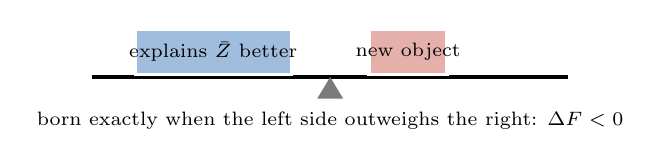
\begin{tikzpicture}[x=0.55cm, y=0.55cm]
    \draw[very thick] (0,0) -- (11,0);
    \fill[muted] (5.5,0) -- (5.2,-0.5) -- (5.8,-0.5) -- cycle;
    \fill[cool!45, draw=white, very thick] (1,0.05) rectangle (4.6,1.1);
    \node[lab] at (2.8,0.58) {explains $\bar Z$ better};
    \fill[accent!40, draw=white, very thick] (6.4,0.05) rectangle (8.2,1.1);
    \node[lab] at (7.3,0.58) {new object};
    \node[lab] at (5.5,-1.0) {born exactly when the left side outweighs the right: $\Delta F<0$};
  \end{tikzpicture}

  \vspace{0.3em}
  \small
  Two models of \emph{different order}, one currency. The complexity is not a penalty added for
  regularisation: it is the same term every live instance already pays.
  \src{agents\_life\_cycle.tex l.594--622}
\end{frame}

\begin{frame}{A streak cannot read evidence}
  \begin{columns}[c]
    \begin{column}{0.52\textwidth}
      \centering
      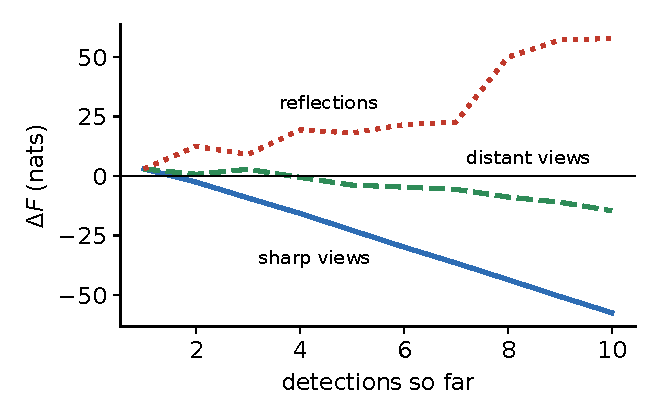
\includegraphics[width=\textwidth]{d3_birth.pdf}
    \end{column}
    \begin{column}{0.45\textwidth}
      \small
      \begin{tabular}{@{}l r r@{}}
        \toprule
        300 runs & streak of 3 & $\Delta F<0$ \\
        \midrule
        2 sharp views & 0\% & 98\% \\
        10 reflections & 94\% & 0\% \\
        \bottomrule
      \end{tabular}

      \vspace{0.8em}
      A streak counts frames. $\Delta F$ reads what each frame says: how sharp it was, and how well
      the frames agree.
    \end{column}
  \end{columns}
  \lesson{Two sharp views are worth more than ten reflections, and only nats can say so.}
  \src{lab 3, exercises 1--2}
\end{frame}

\begin{frame}{What the robot actually computes: a threshold that should not be one}
  \centering
  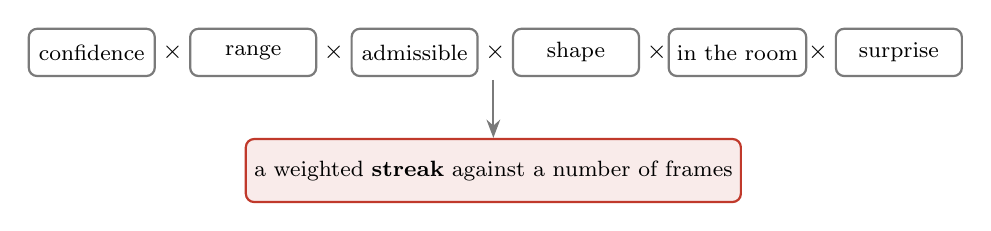
\begin{tikzpicture}[node distance=0.25cm]
    \foreach \t/\x in {confidence/0, range/2.05, admissible/4.1, shape/6.15, in the room/8.2, surprise/10.25}
      \node[bx, draw=muted, minimum width=1.6cm, minimum height=0.6cm] at (\x,0) {\t};
    \foreach \x in {1.025,3.075,5.125,7.175,9.225} \node[font=\small] at (\x,0) {$\times$};
    \node[bx, draw=accent, fill=accent!10, minimum width=4.8cm] (s) at (5.1,-1.5) {a weighted \textbf{streak} against a number of frames};
    \draw[arr, muted] (5.1,-0.35) -- (s);
  \end{tikzpicture}

  \vspace{0.6em}
  \begin{itemize}\small
    \item Every factor stands in for one term of $\Delta F$. As a decomposition it is reasonable.
    \item It loses the \textbf{units}: birth can be traded against nothing else in the model.
    \item Birth and death are decided in \textbf{different currencies}, so a whole subsystem exists
          to undo births that should not have happened.
    \item The proper comparison is within reach; what is missing is plumbing, not theory.
  \end{itemize}
  \src{agents\_life\_cycle.tex l.629--706, l.1276--1282}
\end{frame}

\begin{frame}{The room is the first belief born}
  \begin{columns}[c]
    \begin{column}{0.58\textwidth}
      \small
      \[
        F(m) = \underbrace{\E_q[-\ln p(o\given X,\theta_m,m)]}_{\text{inaccuracy}}
             + \underbrace{\kappa\,|V|}_{\text{complexity}},
        \quad \kappa=\ln\frac{L}{\sigma}
      \]
      \small
      The number of walls is unknown, so the room is a choice of \emph{structure} $m$, priced like
      a birth. One coordinate to $\sigma=3$ cm in a room 10 m across costs
      \[ \ln(10/0.03)\approx 5.8\nats. \]
      Minimum description length and minimum free energy are, here, one rule.
    \end{column}
    \begin{column}{0.38\textwidth}
      \centering
      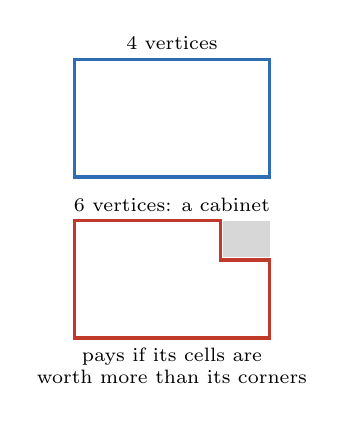
\begin{tikzpicture}[scale=0.62]
        \draw[very thick, cool] (0,0) rectangle (4,2.4);
        \node[lab, above] at (2,2.4) {4 vertices};
        \begin{scope}[shift={(0,-3.3)}]
          \draw[very thick, accent] (0,0) -- (4,0) -- (4,1.6) -- (3,1.6) -- (3,2.4) -- (0,2.4) -- cycle;
          \fill[muted!30] (3.05,1.65) rectangle (4,2.4);
          \node[lab, above] at (2,2.4) {6 vertices: a cabinet};
          \node[lab, below, align=center] at (2,0) {pays if its cells are\\worth more than its corners};
        \end{scope}
      \end{tikzpicture}
    \end{column}
  \end{columns}
  \src{layout\_acquisition.tex l.56--66, l.128--146}
\end{frame}

\begin{frame}{Two regimes, and a loop that is never formed}
  \centering
  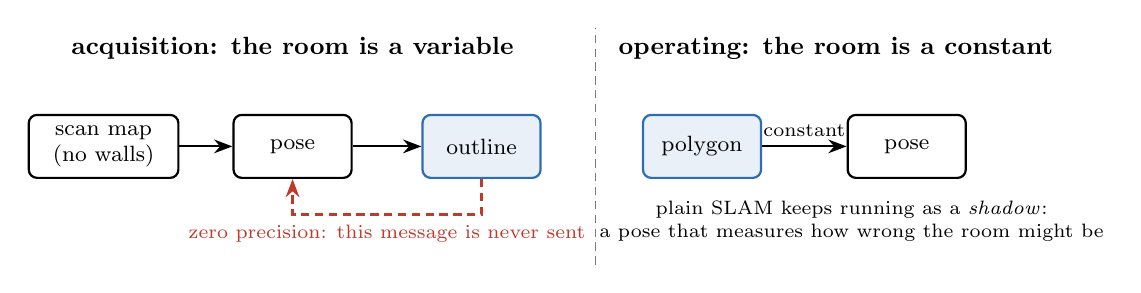
\begin{tikzpicture}
    \node[font=\small\bfseries] at (2.4,1.25) {acquisition: the room is a variable};
    \node[bx, minimum width=1.9cm] (m) at (0,0) {scan map\\(no walls)};
    \node[bx, minimum width=1.5cm] (x) at (2.4,0) {pose};
    \node[bx, draw=cool, fill=cool!10, minimum width=1.5cm] (o) at (4.8,0) {outline};
    \draw[arr] (m) -- (x);
    \draw[arr] (x) -- (o);
    \draw[arr, accent, densely dashed] (o.south) -- ++(0,-0.45) -| node[pos=0.25, below, lab, text=accent] {zero precision: this message is never sent} (x.south);
    \draw[muted, densely dashed] (6.25,-1.5) -- (6.25,1.5);
    \node[font=\small\bfseries] at (9.3,1.25) {operating: the room is a constant};
    \node[bx, draw=cool, fill=cool!10, minimum width=1.5cm] (r) at (7.6,0) {polygon};
    \node[bx, minimum width=1.5cm] (y) at (10.2,0) {pose};
    \draw[arr] (r) -- node[above, lab] {constant} (y);
    \node[lab, align=center] at (9.5,-0.95) {plain SLAM keeps running as a \emph{shadow}:\\a pose that measures how wrong the room might be};
  \end{tikzpicture}

  \vspace{0.5em}
  \begin{itemize}\small
    \item A wrong wall would drag the pose, and the dragged pose would confirm the wrong wall.
    \item One factorised belief, two settings of precision. A room is a slow parameter; a pose is
          a fast state.
    \item The price: a constant cannot be doubted by the localiser that leans on it.
  \end{itemize}
  \src{layout\_acquisition.tex l.162--199}
\end{frame}

\begin{frame}{What tells a wall from a table: free space}
  \begin{columns}[c]
    \begin{column}{0.42\textwidth}
      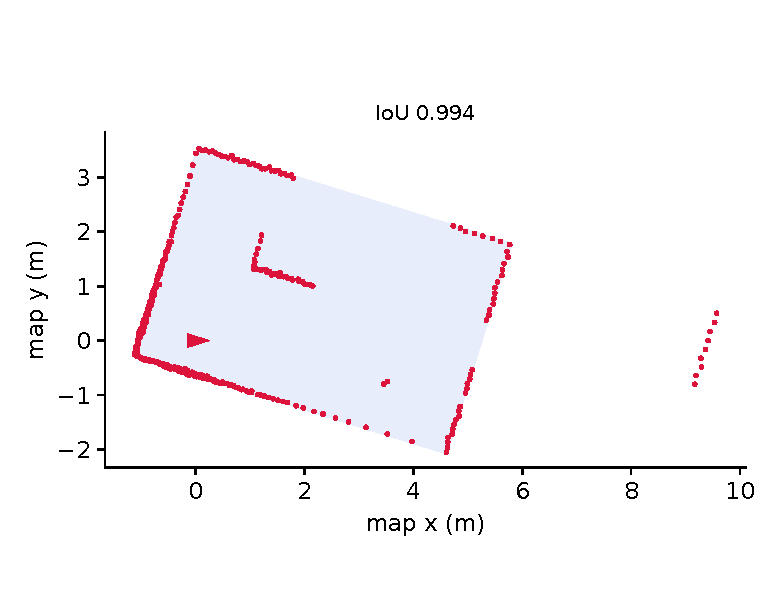
\includegraphics[width=\textwidth]{d3_room.pdf}
    \end{column}
    \begin{column}{0.55\textwidth}
      \small
      In the lab, the table's south face earns \textbf{82 nats} as a candidate wall, against a price
      of 7.6. Evidence for a surface cannot keep furniture out of the room.\\[0.5em]
      The grid therefore keeps two counts per 5 cm cell:
      \[ \text{matter}(c)\iff h_c>n_c \]
      with $h_c$ the beams that stop in the cell and $n_c$ those that pass through it. Only the
      second count can say that a cell is \emph{empty}.\\[0.5em]
      Free floor beyond an edge is evidence against that edge.
    \end{column}
  \end{columns}
  \src{lab 3, exercise 11; layout\_acquisition.tex l.507--526}
\end{frame}

\begin{frame}{A band that is derived, not chosen}
  \begin{columns}[c]
    \begin{column}{0.52\textwidth}
      \small
      Clutter is uniform over $A$. A wall puts its points in a strip $L$ long, $\sigma$ wide:
      \[
        \frac{p_\text{wall}}{p_\text{clutter}} = \frac{A}{L\sqrt{2\pi}\,\sigma}\,e^{-r^2/2\sigma^2}
      \]
      \vspace{-0.6em}
      \begin{itemize}
        \item Inlier iff the ratio exceeds 1: about $3\sigma$.
        \item Each point brings $\ln(\text{ratio})$ \textbf{nats}.
        \item The band \textbf{narrows as $L$ grows}: a long wall is a more expensive explanation.
      \end{itemize}
    \end{column}
    \begin{column}{0.45\textwidth}
      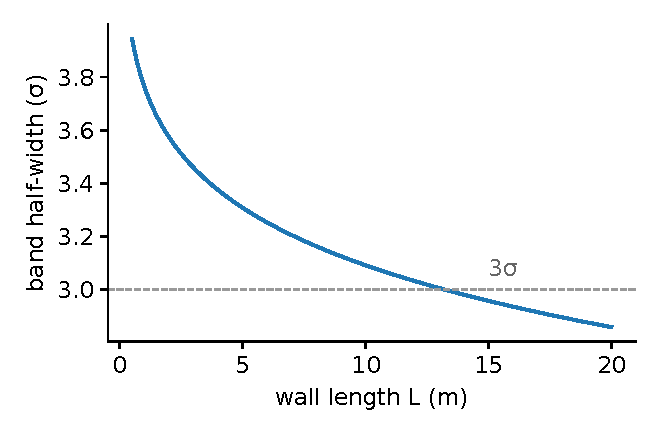
\includegraphics[width=\textwidth]{d3_band.pdf}
    \end{column}
  \end{columns}
  \lesson{A tuned threshold gives the band. The derivation gives the band \emph{and} the currency.}
  \src{lab 3, exercise 8; the same mixture, per cell: layout\_acquisition.tex l.1049--1055}
\end{frame}

\begin{frame}{Promotion: the outline with the shortest description}
  \begin{columns}[c]
    \begin{column}{0.44\textwidth}
      \centering
      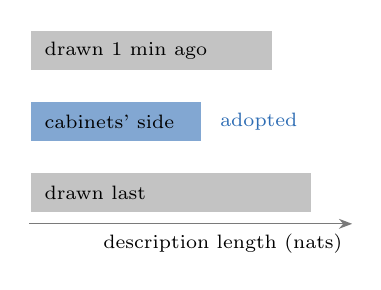
\begin{tikzpicture}[x=1cm, y=1cm]
        \foreach \y/\l/\c/\t in {2.1/3.1/muted!45/{drawn 1 min ago}, 1.2/2.2/cool!60/{cabinets' side}, 0.3/3.6/muted!45/{drawn last}} {
          \fill[\c, draw=white, very thick] (0,\y-0.27) rectangle (\l,\y+0.27);
          \node[lab, anchor=west] at (0.07,\y) {\t};
        }
        \draw[muted, -{Stealth}] (0,-0.1) -- (4.1,-0.1) node[below left, lab, text=black] {description length (nats)};
        \node[lab, anchor=west, text=cool] at (2.3,1.2) {adopted};
      \end{tikzpicture}\\
      {\scriptsize schematic}
    \end{column}
    \begin{column}{0.53\textwidth}
      \small
      The outline moves between wall and furniture as the robot drives, so ``the latest one'' would
      make the room depend on when exploration stopped. Up to 60 recent outlines are kept and
      scored on \emph{all} the evidence.
      \begin{itemize}
        \item In 7 of 10 apartment runs (earlier build) the winner was not the last drawn.
        \item From the kitchen-corner start: overlap 0.968 at promotion, 0.983 refined.
        \item Ten generated rooms: median 0.994.
      \end{itemize}
      {\scriptsize All in simulation; the pipeline has not run on the physical robot.}
    \end{column}
  \end{columns}
  \src{layout\_acquisition.tex l.1036--1046, l.1173--1177, l.1455--1462}
\end{frame}

% =================================================================================================
\section{How a belief ends}
% =================================================================================================

\begin{frame}{A miss is evidence only where the object would have been seen}
  \centering
  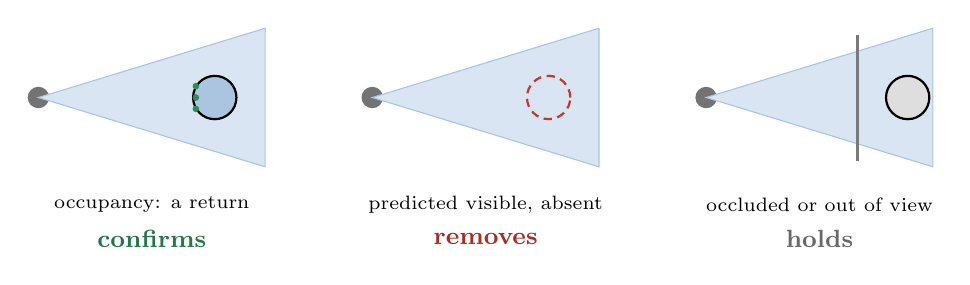
\begin{tikzpicture}[scale=0.8]
    \foreach \x/\t/\c/\v in {0/occupancy: a return/good/confirms, 5.3/{predicted visible, absent}/accent/removes, 10.6/occluded or out of view/muted/holds} {
      \begin{scope}[shift={(\x,0)}]
        \fill[black!55] (0,0.8) circle (0.17);
        \fill[cool!18, draw=cool!40] (0,0.8) -- (3.6,1.9) -- (3.6,-0.3) -- cycle;
        \node[lab, align=center] at (1.8,-0.9) {\t};
        \node[font=\small\bfseries, text=\c!85!black] at (1.8,-1.45) {\v};
      \end{scope}
    }
    \node[obj, fill=cool!40] at (2.8,0.8) {};
    \foreach \y in {0.62,0.8,0.98} \fill[good] (2.5,\y) circle (1.5pt);
    \node[obj, draw=accent, densely dashed] at (8.1,0.8) {};
    \draw[very thick, muted] (13.0,-0.2) -- (13.0,1.8);
    \node[obj, fill=muted!25] at (13.8,0.8) {};
  \end{tikzpicture}

  \vspace{0.8em}
  \small
  The whole stage lies between the middle panel and the right one. Existence is one log-odds $L$
  per instance, clamped to $\pm L_{\max}$, so it stays finite and recoverable.
  \src{agents\_life\_cycle.tex l.887--919}
\end{frame}

\begin{frame}{A factor whose argument list was wrong}
  \begin{columns}[c]
    \begin{column}{0.5\textwidth}
      \centering
      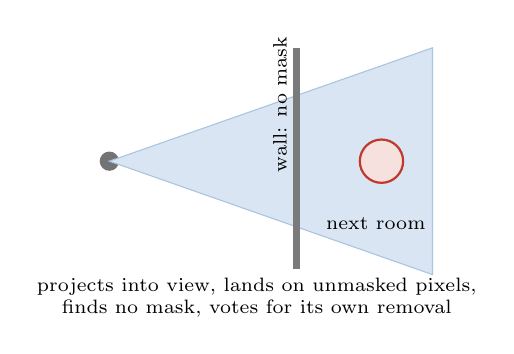
\begin{tikzpicture}[scale=0.72]
        \fill[black!55] (0,0.9) circle (0.17);
        \fill[cool!18, draw=cool!40] (0,0.9) -- (5.7,2.9) -- (5.7,-1.1) -- cycle;
        \draw[line width=2.5pt, muted] (3.3,-1.0) -- (3.3,2.9);
        \node[lab, rotate=90, anchor=south] at (3.3,1.9) {wall: no mask};
        \node[obj, draw=accent, fill=accent!15] at (4.8,0.9) {};
        \node[lab, align=center] at (4.7,-0.2) {next room};
        \node[lab, align=center] at (2.6,-1.5) {projects into view, lands on unmasked pixels,\\finds no mask, votes for its own removal};
      \end{tikzpicture}
    \end{column}
    \begin{column}{0.47\textwidth}
      \small
      \[
        P(M\given\theta,\ell,X)\ \longrightarrow\ P(M\given\theta,\ell,X,\alert{\mathcal R})
      \]
      A wall is not a detector class, so without the room polygon every wall is transparent.\\[0.5em]
      \begin{measured}{the same defect, three agents}
        Refrigerator, then door, then table and cabinet. Each copy was consistent with itself, so
        no per-agent test could find it.
      \end{measured}
    \end{column}
  \end{columns}
  \src{agents\_life\_cycle.tex l.921--951; CONCEPT\_AGENT\_LIFECYCLE.md l.7--11}
\end{frame}

\begin{frame}{Weight absence by $P(\text{detect})$, on the correct side of the ceiling}
  \centering
  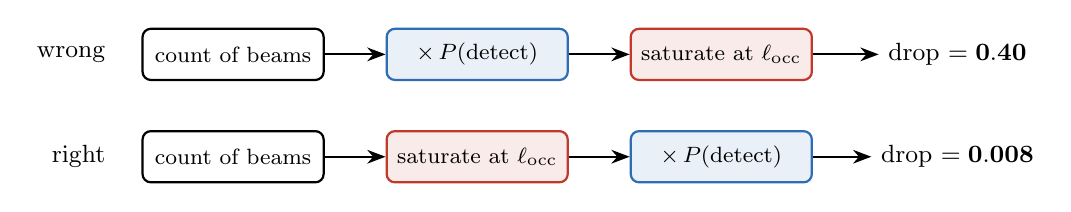
\begin{tikzpicture}
    \tikzset{st/.style={bx, minimum width=2.3cm, minimum height=0.65cm}}
    \node[anchor=east, font=\small] at (-1.5,0) {wrong};
    \node[st] (a1) at (0,0) {count of beams};
    \node[st, draw=cool, fill=cool!10] (a2) at (3.1,0) {$\times\,P(\text{detect})$};
    \node[st, draw=accent, fill=accent!10] (a3) at (6.2,0) {saturate at $\ell_\text{occ}$};
    \node[font=\small] (a4) at (9.2,0) {drop $=\mathbf{0.40}$};
    \draw[arr] (a1) -- (a2); \draw[arr] (a2) -- (a3); \draw[arr] (a3) -- (a4);
    \node[anchor=east, font=\small] at (-1.5,-1.3) {right};
    \node[st] (b1) at (0,-1.3) {count of beams};
    \node[st, draw=accent, fill=accent!10] (b2) at (3.1,-1.3) {saturate at $\ell_\text{occ}$};
    \node[st, draw=cool, fill=cool!10] (b3) at (6.2,-1.3) {$\times\,P(\text{detect})$};
    \node[font=\small] (b4) at (9.2,-1.3) {drop $=\mathbf{0.008}$};
    \draw[arr] (b1) -- (b2); \draw[arr] (b2) -- (b3); \draw[arr] (b3) -- (b4);
  \end{tikzpicture}

  \vspace{0.6em}
  {\small A view in which a present object would be only 2\% resolvable.}

  \lesson{A modulation applied upstream of a saturation is invisible: the saturation absorbs it.}
  \src{agents\_life\_cycle.tex l.953--973; numbers: lab 3, exercise 4}
\end{frame}

\begin{frame}{Four rules, one tour}
  \begin{columns}[c]
    \begin{column}{0.46\textwidth}
      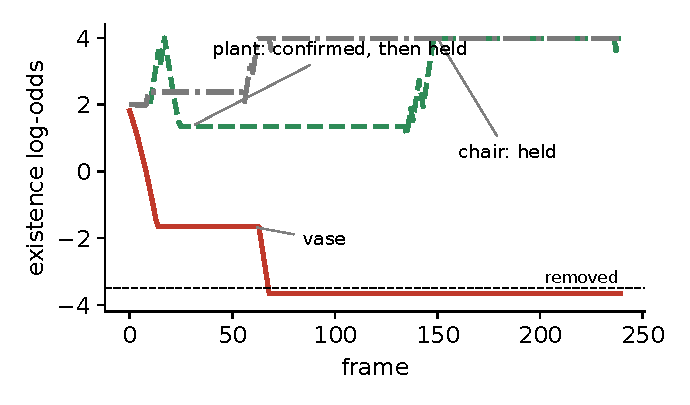
\includegraphics[width=\textwidth]{d3_existence.pdf}
    \end{column}
    \begin{column}{0.51\textwidth}
      \footnotesize
      \begin{tabular}{@{}l l@{}}
        \toprule
        rule & removes (frame) \\
        \midrule
        \textbf{evidence} & vase (68) \\
        no walls in line of sight & vase (68), \alert{chair} (174) \\
        weight the count & vase (13) \\
        miss counter & \alert{everything} by frame 44 \\
        \bottomrule
      \end{tabular}

      \vspace{0.6em}
      \small
      Never resolvable? No decay constant. The instance is routed to a \textbf{verification
      pull}: uncertainty that cannot be resolved from here is a reason to move.
    \end{column}
  \end{columns}
  \src{lab 3, exercise 4; agents\_life\_cycle.tex l.975--985}
\end{frame}

% =================================================================================================
\section{How a belief fades}
% =================================================================================================

\begin{frame}{A constant $Q$ forgets on the agent's clock}
  \begin{columns}[c]
    \begin{column}{0.47\textwidth}
      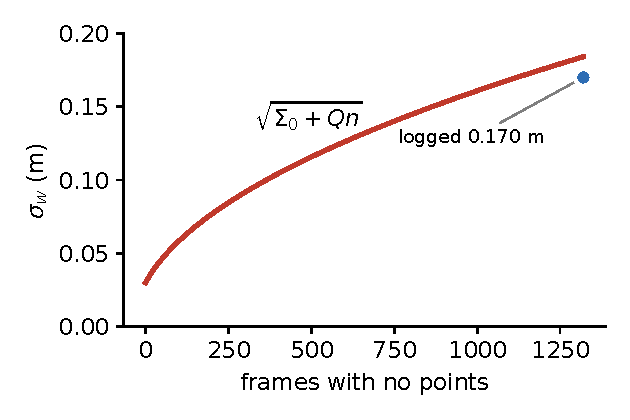
\includegraphics[width=\textwidth]{d3_constq.pdf}
    \end{column}
    \begin{column}{0.5\textwidth}
      \small
      $\Sigma\leftarrow\Sigma+Q$, every frame, seen or not, with $Q=(0.005\text{ m})^2$.
      \begin{itemize}
        \item A converged table ($\sigma_w\approx 3$ cm) loses half its precision in
              \textbf{3.6 s}.
        \item It is back at the prior after about \textbf{5.9 minutes}, whether it was tracked for
              thirty seconds or for three hours.
      \end{itemize}
      \begin{measured}{a real table, 1320 blind cycles}
        Predicted $\sigma_w = 0.184$ m; logged $0.170$ m. The next sparse mask re-cut the table.
      \end{measured}
    \end{column}
  \end{columns}
  \src{agents\_life\_cycle.tex l.1007--1043}
\end{frame}

\begin{frame}{Observed, precision stops at a floor}
  One predict plus one update, $\Sigma^{-1}\leftarrow\Sigma^{-1}+i$, with $y$ the predicted precision and
  $\varrho=Q$:
  \[
    \frac1y=\frac1{y+i}+\varrho
    \quad\Longrightarrow\quad
    \boxed{\;\sigma_\text{steady}\approx(\varrho/i)^{1/4}\;}
  \]
  \begin{itemize}
    \item \alert{Elapsed time does not appear.} Evidence is discarded at the rate it is acquired:
          three hours of observation leave the belief where thirty seconds did.
    \item Lab: formula 10.0 mm, simulated 9.4 mm.
    \item Clamping $\Sigma$ caps the first problem and does nothing about this one.
  \end{itemize}
  \lesson{Nothing an agent learns extends how long it stays resistant.}
  \src{agents\_life\_cycle.tex l.1045--1082; lab 3, exercise 5}
\end{frame}

\begin{frame}{A constant becomes an inferred quantity}
  Each instance carries a log-volatility, $Q=e^{\zeta}$, driven by its own surprise:
  \[
    \zeta \leftarrow \zeta + \eta\Big(
      \underbrace{\tfrac12\,\tilde d-\tfrac12\E[\tilde d\,]}_{\text{surprise seen minus expected}}
      - \underbrace{\frac{\zeta-\zeta_0}{\sigma_\zeta^2}}_{\text{hyperprior pull-back}}\Big)
  \]
  \begin{columns}[T]
    \begin{column}{0.5\textwidth}
      \small
      \begin{itemize}
        \item Consistent views: $\zeta$ falls, memory lengthens, precision accumulates.
        \item A sustained surprise: $\zeta$ rises and the model adapts. Stiffness is never a lock.
      \end{itemize}
    \end{column}
    \begin{column}{0.46\textwidth}
      \small
      In the lab $\tilde d$ is the saturating (Student-$t$) surprise of the innovation: one
      outrageous frame moves $\zeta$ by a bounded amount.\\[0.3em]
      \alert{Design only: no agent runs this yet.}
    \end{column}
  \end{columns}
  \src{agents\_life\_cycle.tex l.1085--1125 (form of the update); lab 3, exercise 5}
\end{frame}

\begin{frame}{In the toy: stiff, but not locked}
  \begin{columns}[c]
    \begin{column}{0.56\textwidth}
      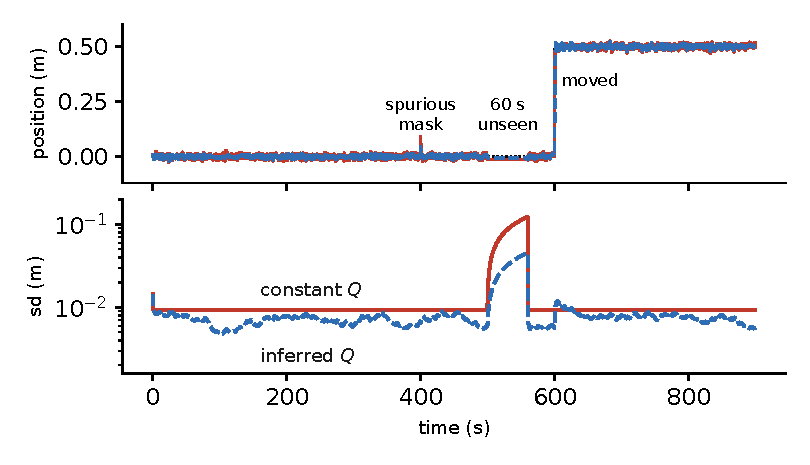
\includegraphics[width=\textwidth]{d3_volatility.pdf}
    \end{column}
    \begin{column}{0.41\textwidth}
      \footnotesize
      \begin{tabular}{@{}l r r@{}}
        \toprule
         & constant & inferred \\
        \midrule
        sd before (mm) & 9.4 & 6.5 \\
        spurious mask (mm) & 92 & 44 \\
        after 60 s unseen (mm) & 123 & 45 \\
        frames to adapt & 9 & 15 \\
        \bottomrule
      \end{tabular}

      \vspace{0.6em}
      \small
      The failure mode: a steady \textbf{bias} looks like agreement. A 5 cm bias ends $5.4\sigma$
      out with constant $Q$, $7.6\sigma$ with inferred.
    \end{column}
  \end{columns}
  \src{lab 3, exercises 5--6; agents\_life\_cycle.tex l.1127--1133}
\end{frame}

% =================================================================================================
\section{Localisation is one more belief}
% =================================================================================================

\begin{frame}{The room supplies the likelihood}
  \begin{columns}[c]
    \begin{column}{0.58\textwidth}
      \small
      For a scan $\{p_i\}$ and a candidate pose $X$:
      \[
        d_i(X)=\operatorname{dist}\big(R(\phi)p_i+t,\ \mathcal R\big)
      \]
      \[
        \mathcal L_\text{obs}=\frac{1}{2\sigma^2}\cdot\frac1N\sum_i w_i\,\mathrm{Huber}(d_i)
      \]
      \begin{itemize}
        \item The residual \emph{is} the prediction error: no expected scan is rendered.
        \item Note the $\frac1N$: the precision does not grow with scan density.
        \item Range and incidence weights are precisions on a covariate, not gates.
      \end{itemize}
    \end{column}
    \begin{column}{0.4\textwidth}
      \centering
      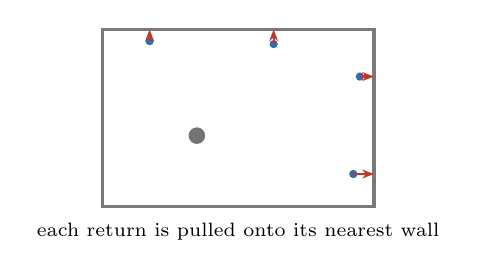
\begin{tikzpicture}[scale=0.75]
        \draw[very thick, muted] (0,0) rectangle (4.6,3);
        \fill[black!55] (1.6,1.2) circle (0.14);
        \foreach \px/\py/\qx/\qy in {4.36/2.2/4.6/2.2, 4.25/0.55/4.6/0.55, 2.9/2.75/2.9/3, 0.8/2.8/0.8/3} {
          \fill[cool] (\px,\py) circle (2pt);
          \draw[accent, thick, -{Stealth[length=1.5mm]}] (\px,\py) -- (\qx,\qy);
        }
        \node[lab, align=center] at (2.3,-0.42) {each return is pulled onto its nearest wall};
      \end{tikzpicture}
    \end{column}
  \end{columns}
  \src{room\_concept.tex l.243--307}
\end{frame}

\begin{frame}{What the residual floor is made of}
  \begin{columns}[c]
    \begin{column}{0.36\textwidth}
      \centering
      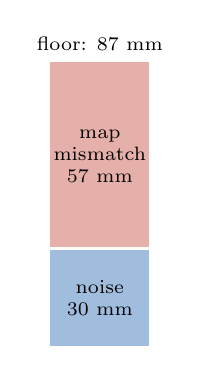
\begin{tikzpicture}[y=0.042cm, x=1cm]
        \fill[cool!45, draw=white, very thick] (0,0) rectangle (1.3,30);
        \fill[accent!40, draw=white, very thick] (0,30) rectangle (1.3,87);
        \node[lab, align=center] at (0.65,15) {noise\\30 mm};
        \node[lab, align=center] at (0.65,58) {map\\mismatch\\57 mm};
        \node[lab, above] at (0.65,87) {floor: 87 mm};
      \end{tikzpicture}
    \end{column}
    \begin{column}{0.6\textwidth}
      Park the robot. The mean wall distance of each scan hovers near 87 mm and never reaches zero.
      \begin{itemize}\small
        \item Its fluctuation is white: $N^{-1/2}$, measured ratio $1.41$ against a predicted
              $\sqrt{405/200}=1.42$.
        \item That fixes the per-point scatter at $\approx 37$ mm, which explains
              $0.798\times 37\approx 30$ mm.
      \end{itemize}
    \end{column}
  \end{columns}
  \lesson{Two-thirds of the floor is an error every return shares. More returns cannot remove it.}
  \src{room\_concept.tex l.386--426}
\end{frame}

\begin{frame}{Localising against the room you just built}
  \begin{columns}[c]
    \begin{column}{0.46\textwidth}
      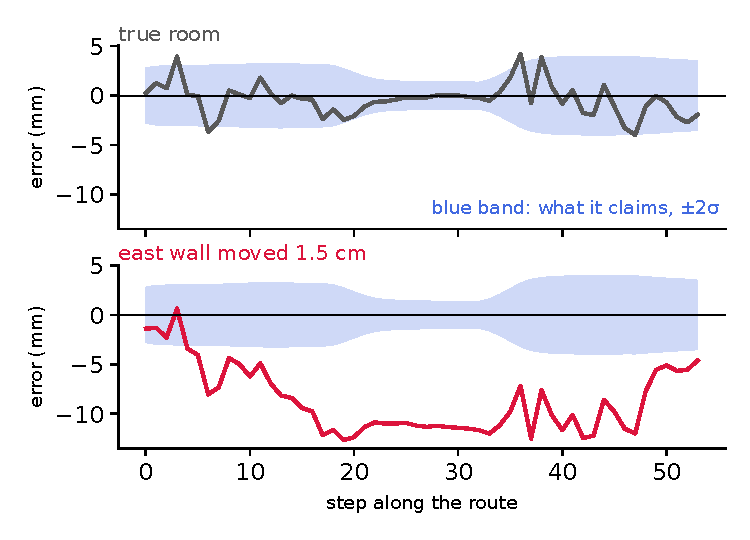
\includegraphics[width=\textwidth]{d3_track.pdf}
    \end{column}
    \begin{column}{0.42\textwidth}
      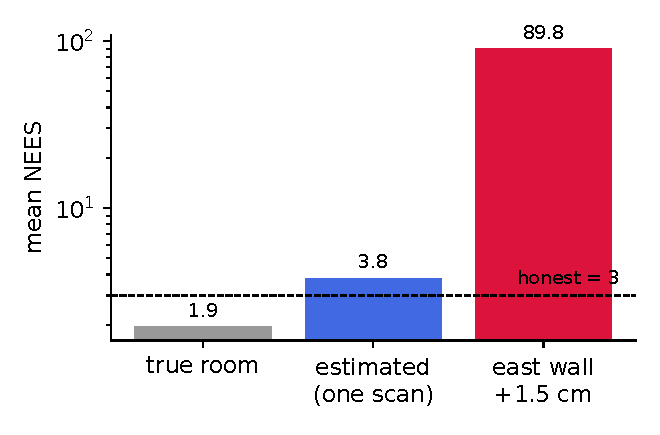
\includegraphics[width=\textwidth]{d3_nees.pdf}
      \small
      A wall \textbf{1.5 cm} out of place makes the localiser confidently wrong: NEES 90 where 3 is
      honest.
    \end{column}
  \end{columns}
  \lesson{In the operating regime the polygon is a constant, so its error is shared by every scan,
          for ever.}
  \src{lab 3, exercise 13}
\end{frame}

\begin{frame}{Symmetry: where descent cannot help}
  \begin{columns}[c]
    \begin{column}{0.45\textwidth}
      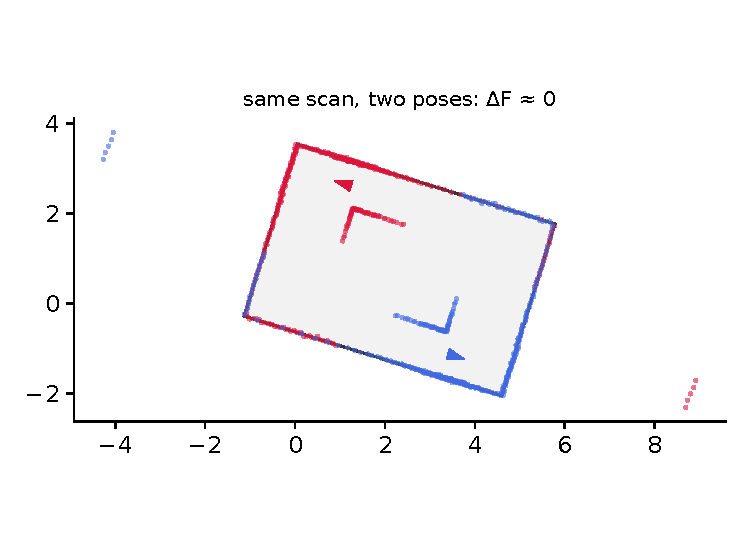
\includegraphics[width=\textwidth]{d3_symmetry.pdf}
    \end{column}
    \begin{column}{0.53\textwidth}
      \small
      A rectangle looks the same after a half-turn: the same scan fits both poses with
      \emph{identical} free energy, and no downhill path joins them.\\[0.5em]
      They are separate hypotheses, so the agent enumerates them and chooses: a discrete search,
      then local refinement.\\[0.5em]
      This is one of the few places where a threshold is right:
      \alert{a threshold is defensible exactly when the alternative cannot be expressed as a
      covariance.}
    \end{column}
  \end{columns}
  \src{room\_concept.tex l.1869--1927}
\end{frame}

% =================================================================================================
\section{Whose evidence is it?}
% =================================================================================================

\begin{frame}{Association: the factor the free energy cannot see}
  \begin{columns}[c]
    \begin{column}{0.46\textwidth}
      \centering
      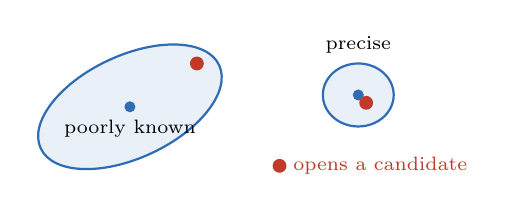
\begin{tikzpicture}
        \draw[cool, thick, fill=cool!10, rotate around={25:(0,0)}] (0,0) ellipse (1.25 and 0.65);
        \fill[cool] (0,0) circle (2pt); \node[lab, below] at (0,-0.05) {poorly known};
        \draw[cool, thick, fill=cool!10] (2.9,0.15) ellipse (0.45 and 0.4);
        \fill[cool] (2.9,0.15) circle (2pt); \node[lab, above] at (2.9,0.55) {precise};
        \fill[accent] (0.85,0.55) circle (2.5pt);
        \fill[accent] (3.0,0.05) circle (2.5pt);
        \fill[accent] (1.9,-0.75) circle (2.5pt);
        \node[lab, right, text=accent] at (1.95,-0.75) {opens a candidate};
      \end{tikzpicture}\\[0.4em]
      {\small a poorly known instance accepts detections from further away}
    \end{column}
    \begin{column}{0.51\textwidth}
      \small
      \[
        P(M\given X,Z,\Phi)\approx\mathbf 1[M=\hat M],\quad
        S=\Sigma^{xy}_{\theta_i}+\sigma_\text{det}^2 I
      \]
      Squared Mahalanobis distance at most 9, assigned greedily, lowest cost first.\\[0.5em]
      A distribution on one value has no entropy and no expectation: the matching is free, in the
      literal sense that $F$ cannot see it. \alert{A wrong match is invisible to the quantity that
      would have registered it.}\\[0.5em]
      The repair comes later and from elsewhere: merging, and the existence belief.
    \end{column}
  \end{columns}
  \src{concept\_agents.tex l.483--486, l.859--889}
\end{frame}

\begin{frame}{A mask is a qualified likelihood}
  \centering
  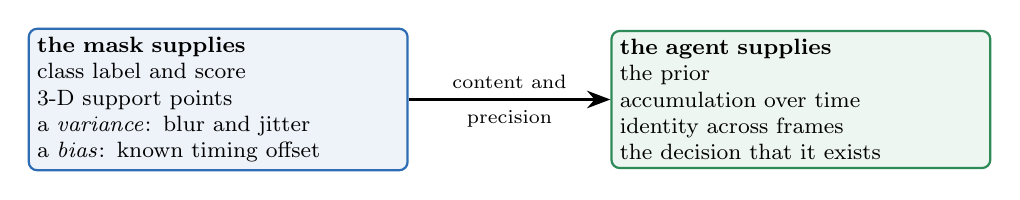
\begin{tikzpicture}
    \node[bx, draw=cool, fill=cool!8, text width=4.6cm, align=left] (m) at (0,0) {\textbf{the mask supplies}\\
      class label and score\\3-D support points\\a \emph{variance}: blur and jitter\\a \emph{bias}: known timing offset};
    \node[bx, draw=good, fill=good!8, text width=4.6cm, align=left] (a) at (7.4,0) {\textbf{the agent supplies}\\
      the prior\\accumulation over time\\identity across frames\\the decision that it exists};
    \draw[arr, very thick] (m) -- node[above, lab] {content and} node[below, lab] {precision} (a);
  \end{tikzpicture}

  \vspace{0.7em}
  \begin{itemize}\small
    \item The producer reports the physics of capture; the consumer decides what that does to
          its belief. The hub gates nothing.
    \item Variance and bias are published separately because they are different:
          \alert{symmetric error downweights, biased error gates.}
    \item The qualification is a prior on the \emph{channel}, not on the world.
  \end{itemize}
  \src{phylogenetic\_perception.tex l.347--408}
\end{frame}

% =================================================================================================
\section{Shared error}
% =================================================================================================

\begin{frame}{The common-mode ceiling}
  $N$ residuals that share one offset $\delta\sim\N(0,\Sigma_\delta)$, a pose error, plus independent
  noise. Marginalise $\delta$:
  \[
    \mathcal I = J_z^\top\big(\sigma^2 I + J_z\Sigma_\delta J_z^\top\big)^{-1}J_z
    \;\overset{\text{Woodbury}}{=}\;
    \big(\sigma^2(J_z^\top J_z)^{-1} + \Sigma_\delta\big)^{-1}
    \;\xrightarrow[N\to\infty]{}\; \Sigma_\delta^{-1}
  \]
  \begin{itemize}
    \item A denser mask eventually stops helping. The ceiling is set by the \emph{pose} error, not
          by the pixel count.
    \item The joint information on (object, offset) has rank 6, not 12: the data cannot tell a
          displaced object from a displaced robot.
  \end{itemize}
  \src{concept\_agents.tex l.1048--1090}
\end{frame}

\begin{frame}{The ceiling, measured in the toy}
  \begin{columns}[c]
    \begin{column}{0.48\textwidth}
      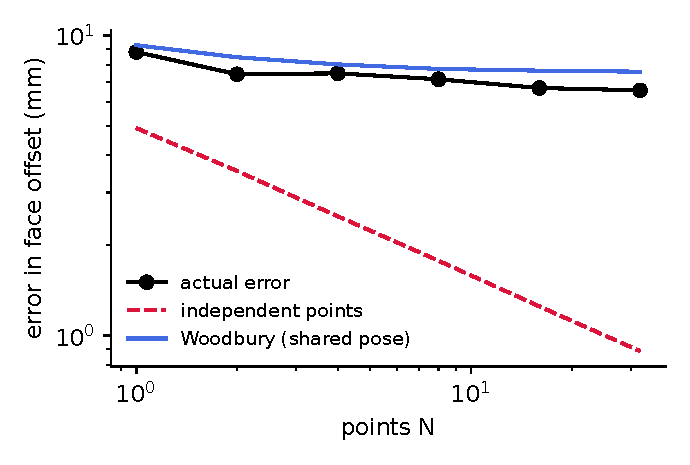
\includegraphics[width=\textwidth]{d3_ceiling.pdf}
    \end{column}
    \begin{column}{0.5\textwidth}
      \small
      The robot maps the table's face from a \emph{dead-reckoned} pose.
      \begin{itemize}
        \item Treating points as independent claims under 1 mm at $N=32$.
        \item The real error stalls near 7 mm.
        \item Woodbury predicts it to within about 15\% at every $N$.
      \end{itemize}
    \end{column}
  \end{columns}
  \lesson{Averaging removes independent error. It does not remove shared error.}
  \src{lab 3, exercise 15}
\end{frame}

\begin{frame}{Case study: association dies by a common-mode latch \wip}
  \begin{columns}[T]
    \begin{column}{0.5\textwidth}
      \small One frame of a real recording, on an earlier estimator:\\[0.3em]
      \footnotesize
      \begin{tabular}{@{}c r r r@{}}
        \toprule
        seg & $\chi^2$ & $\Delta\phi$ & gate $\sigma_\phi$ \\
        \midrule
        0 & 1.03 & $-5.85^\circ$ & $6.78^\circ$ \\
        1 & 1.02 & $-5.76^\circ$ & $6.34^\circ$ \\
        2 & 1.20 & $-5.79^\circ$ & $6.01^\circ$ \\
        3 & 1.06 & $-5.77^\circ$ & $6.67^\circ$ \\
        \bottomrule
      \end{tabular}
    \end{column}
    \begin{column}{0.48\textwidth}
      \small
      The \emph{same} $-5.8^\circ$ on every wall is one \textbf{heading} error, not four wall
      errors.\\[0.5em]
      Each wall is gated independently against an error they all share. When it crosses
      $\approx 6^\circ$ they all fail \alert{in the same frame}, nothing is left to correct the
      pose, and association goes from 100\% to 0\% for ever.
    \end{column}
  \end{columns}
  \vspace{0.4em}
  \small ``A parked run looks perfect and the first tour kills it.''
  \src{post-thesis note, 2026-09-18}
\end{frame}

% =================================================================================================
\section{Lab}
% =================================================================================================

\begin{frame}{Lab 3: a belief's life, and what it stands on}
  \texttt{labs/day3.ipynb}, about two hours.
  \begin{columns}[T]
    \begin{column}{0.48\textwidth}
      \small
      \textbf{How a belief begins and ends}
      \begin{enumerate}
        \item[A.] \textbf{Birth}: $\Delta F$ against a streak of three.
        \item[B.] \textbf{Absence}: line of sight through walls; the weight after the ceiling; four
                  rules on one tour.
        \item[C.] \textbf{Forgetting}: constant $Q$ against inferred volatility; then a bias.
      \end{enumerate}
    \end{column}
    \begin{column}{0.48\textwidth}
      \small
      \textbf{What it stands on}
      \begin{enumerate}
        \item[D.] \textbf{The room}: the vote, the band, four walls; does the table pay the price?
        \item[E.] \textbf{The pose}: drive the route; NEES on three maps.
        \item[F.] \textbf{Symmetry}: $F$ at the true pose and its half-turn.
        \item[G.] \textbf{Ceiling}: independent against Woodbury.
      \end{enumerate}
    \end{column}
  \end{columns}
  \vspace{0.5em}
  \small Short of time: A, B, C, E and G.
\end{frame}

\begin{frame}{Tomorrow}
  \begin{columns}[c]
    \begin{column}{0.55\textwidth}
      Today the robot watched. Tomorrow it decides:
      \begin{itemize}
        \item objects publish what they can do for its uncertainty, priced in nats;
        \item expected free energy chooses, and where to look next is experiment design;
        \item routes and tracking become control problems with no separate obstacle term;
        \item and it turns the same objective on itself: calibration as inference.
      \end{itemize}
    \end{column}
    \begin{column}{0.42\textwidth}
      \begin{block}{Reading for Day 4}\small
        Thesis chapters:
        \begin{itemize}
          \item \emph{Action: affordances and the expected free energy}, up to ``Why the gradient
                decomposes'';
          \item \emph{Self-Calibration of the Robot's Body}: ``What the body is'', ``What no data
                can determine'', ``What each motion makes observable''.
        \end{itemize}
      \end{block}
    \end{column}
  \end{columns}
\end{frame}

\end{document}
